\ifx\wholebook\relax \else

\documentclass[b5paper]{ctexart}
\usepackage[nomarginpar
  %, margin=.5in
]{geometry}

\addtolength{\oddsidemargin}{-0.05in}
\addtolength{\evensidemargin}{-0.05in}
\addtolength{\textwidth}{0.1in}

\usepackage[cn]{../prelude}

\setcounter{page}{1}

\begin{document}

\title{数的诞生}

\author{刘新宇
\thanks{{\bfseries 刘新宇} \newline
  Email: liuxinyu99@hotmail.com \newline}
  }

\maketitle
\fi

\markboth{数的诞生}{数的旅程}

\ifx\wholebook\relax
\chapter{数的诞生}
\numberwithin{Exercise}{chapter}
\fi

\epigraph{一二三四五,金木水火土。\\ 
天地分上下,日月照今古。}{部编小学一年级\\
语文课本第一课}

数充满了我们的生活。例如报纸上这段新闻报道:“2024年巴黎奥运会(第33届奥运会)已于当地时间2024年8月1日闭幕。巴黎是继伦敦后的世界第2个至少3次举办夏奥会的城市。这是首届男女比例完全平衡的奥运会,男女运动员各为5250名。本届奥运会共设有32个大项,329个小项,共有206个国家和地区参赛,新增了滑板、冲浪、竞技攀岩和霹雳舞四个大项。中国代表团最终在巴黎奥运会上夺得40金27银24铜的优异成绩。”

这短短的180字中有14个数字。数是谁发明的?历史书上没有答案。数出现在所有历史文字记录中,数也许诞生在史前,伴随着语言和文字。要找到答案,我们有两条线索:1、追寻古老的历史物证,石刻、壁画、器物上关于数的印记;2、追溯数在语言演变中的痕迹。比如英文中的eleven (11)来自古英语endleofan,意思是(数到10还)剩余1;tweleve (12)来自twelf,意思是剩余2。

\section{罗塞塔石碑}

走进大英博物馆第4展厅,有一件展品吸引着观众。这是一块残缺的石碑,长114厘米,宽72厘米,上面刻满了文字(\cref{fig:rosetta-stone})。人们能一眼辨认出有一部分是希腊字母(\cref{fig:rosetta-greek},参见\cref{ch:greek-letters}希腊字母表),但剩下的部分犹如天书。仔细观察会发现余下的文字大致分成两种,一种是弯弯曲曲的符号,如\cref{fig:rosetta-demotic},另一种是奇妙的图案,如\cref{fig:rosetta-hieroglyphs}。

这一展品叫做罗塞塔石碑。1799年法军远征埃及。拿破仑还随军带有一群厉害的数学家。这位未来的法兰西皇帝,从一名炮兵军官脱颖而出。他敏锐地看出数学不仅可以算出大炮的弹道,还关乎法兰西的国运。7月15日,一位士兵在尼罗河三角洲前线的小镇罗塞塔(Rosetta)发掘防御工事。他偶然发现了一块断碑砌在一段古老的墙中。尽管并不完整(如\cref{fig:rosetta-stone-recons}),这仍是一个重大的发现。1801年,英军击败了拿破仑,罗塞塔石碑也落入了英军之手。1802年2月,它被运抵英国朴次茅斯港,并最终收藏于大英博物馆。

\begin{figure}[htbp]
 \centering
 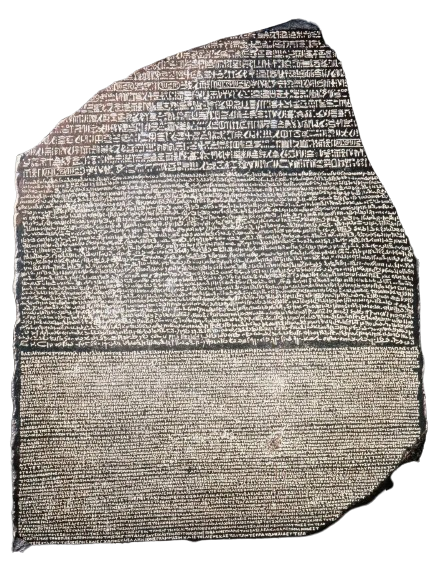
\includegraphics[scale=0.4]{img/rosetta-stone}
 \caption{罗赛塔石碑,古埃及,公元前196年}
 \label{fig:rosetta-stone}
\end{figure}

\begin{figure}[htbp]
  \centering
  \subcaptionbox{古希腊文,共54行\label{fig:rosetta-greek}}{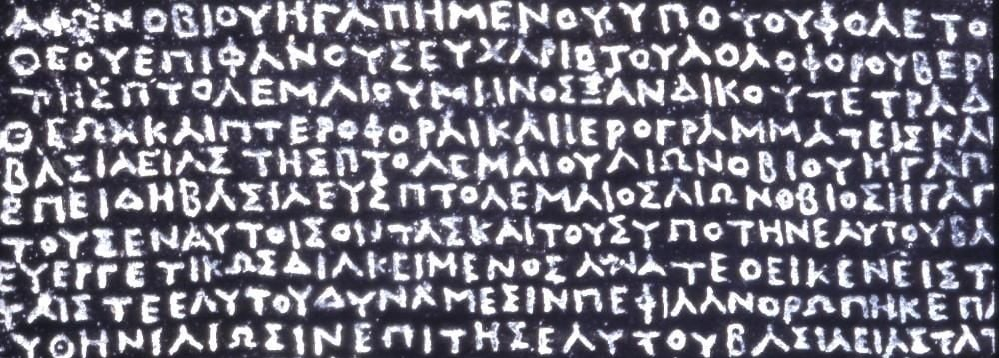
\includegraphics[scale=0.6]{img/Rosetta-Greek}} \\
  \subcaptionbox{古埃及世俗文字,共32行\label{fig:rosetta-demotic}}{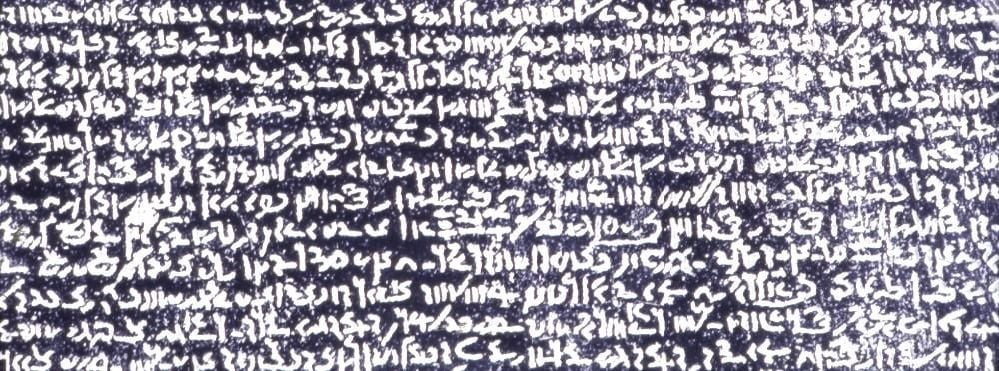
\includegraphics[scale=0.6]{img/Rosetta-Demotic}} \\
  \subcaptionbox{古埃及象形文字,共14行\label{fig:rosetta-hieroglyphs}}{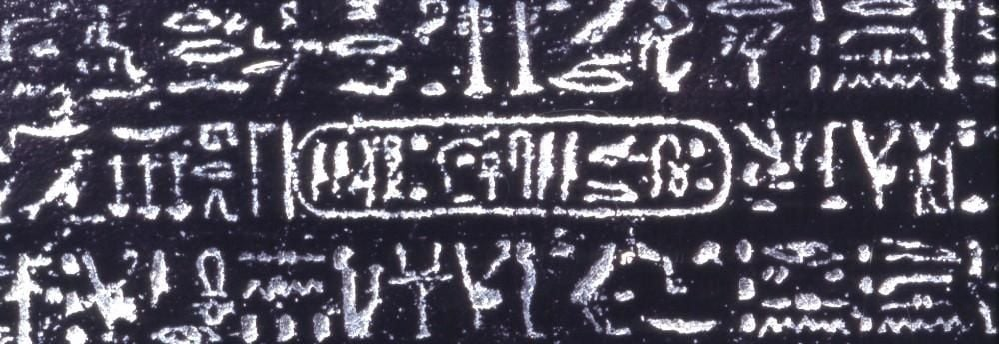
\includegraphics[scale=0.6]{img/Rosetta-Hieroglyphs}}
  \caption{罗赛塔石碑上的三种文字}
  \label{fig:rosetta-stone}
 \end{figure}
 
 \begin{figure}[htbp]
  \centering
  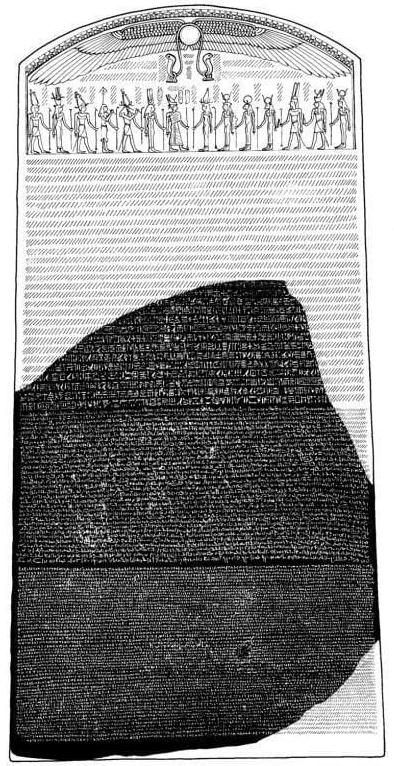
\includegraphics[scale=0.4]{img/Rosetta-stone-recons}
  \caption{罗赛塔石碑并不完整,从中间断裂。}
  \label{fig:rosetta-stone-recons}
 \end{figure}

\ifx\wholebook\relax \else
\section{参考答案}
\shipoutAnswer

\begin{thebibliography}{99}

%% \bibitem{wiki-number}
%% Wikipedia. ``古代计数系统的历史''. \url{https://en.wikipedia.org/wiki/History_of_ancient_numeral_systems}

%% \bibitem{trip-to-number-kingdom}
%% [美]\ 卡尔文$\cdot$C$\cdot$克劳森\ 著\ 袁向东、袁钧\ 译. ``数学旅行家:漫游数王国''. 上海教育出版社。ISBN: 7-5320-7883-3/G $\cdot$ 7972

%% \bibitem{wiki-babylonian-num}
%% Wikipedia. ``古巴比伦数字''. \url{https://en.wikipedia.org/wiki/Babylonian_numerals}

\end{thebibliography}

\expandafter\enddocument
%\end{document}

\fi
